\chapter{Гипотеза де Бройля и её экспериментальное подтверждение. 
Корпускулярно-волновой дуализм свойств вещества. Опыты Девиссона-
Джермера и Томсона. Волновая функция. Статистическая интерпретация 
волн де Бройля и волновой функции. Соотношение неопределенностей.}

В 1924(27) г. Луи де Бройль обобщил корпускулярно-волновой дуализм на все
частицы материи. Он выдвинул гипотезу, согласно которой каждой частице можно
поставить в соответствие некоторый волновой процесс (т.е он не говорит, что
частица -- это волна, он лишь проводит соответствие), длина волны которого
\[
    \lambda_\text{Б} = \frac{h}{p} = \frac{h}{mv}.
\]
Эти волны назвали волнами де Бройля.


\section{Опыт Дэвиссона-Джермера}
\begin{figure}[h!]
    \center
    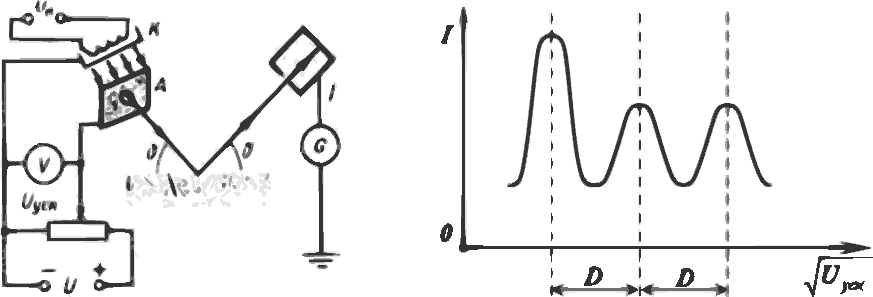
\includegraphics[width=.47\textwidth]{05-Davisson_Germer_experiment_1}\hfill
    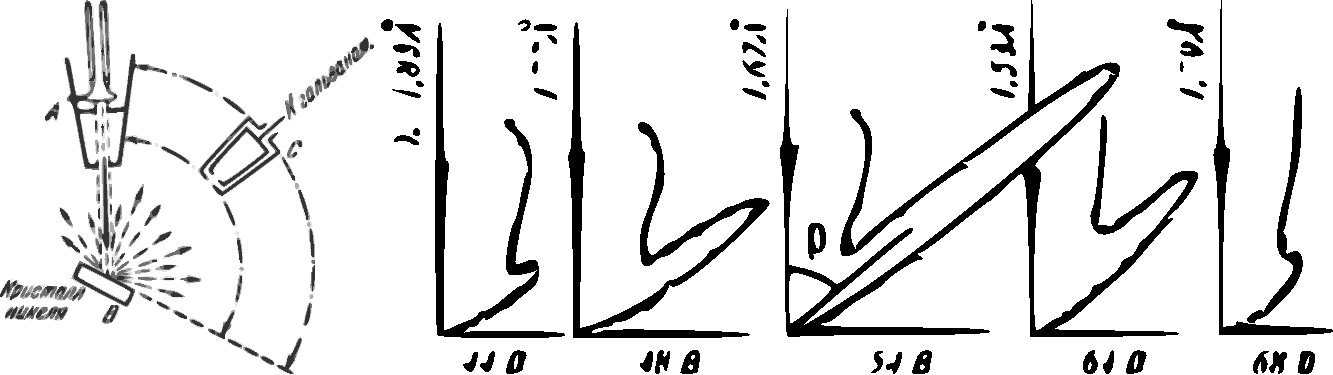
\includegraphics[width=.47\textwidth]{05-Davisson_Germer_experiment_2}
\end{figure}
Схема установки аналогична схеме по изучению дифракции рентгеновских лучей на
кристалле.
\begin{align*}
    \frac{mv^2}{2} = eU, & v = \sqrt{\frac{2eU}{m}},
    & \lambda_\text{Б} = \frac{h}{\sqrt{2eUm}}.
\end{align*}
Если пучок обладает волновыми свойствами, то должна наблюдаться дифракция в
соответствии с законом Вульфа-Брегга:
\begin{align*}
    & 2d\sin\theta = n\lambda,
    & \lambda = \frac{2d\sin\theta}{n}.
\end{align*}
\[
    n = 1, d = 0.0929 нм,  \theta = 64^\circ, U = 54 В
\]
Значения, вычисленные по гипотезе де Бройля совпали с результатами, полученными
из формулы Брегга-Вульфа.

Полученные кривые зависимостей интенсивности отражённого пучка при различных
углах наблюдения имели немонотонный характер -- у них имелись максимумы и
минимумы, что подтверждало волновые свойства пучка.

\section{Тартаковский и Томсон}
Суть эксперимента и его результаты показаны на рисунке~\ref{fig:05-Thomson_experiment}.
\begin{figure}[h!]
    \center
    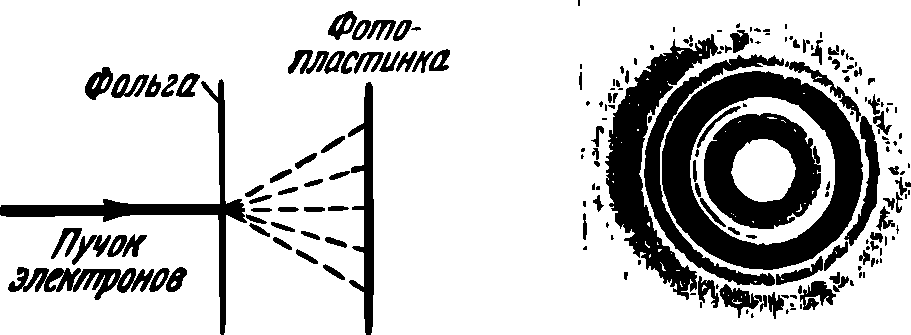
\includegraphics[width=.5\textwidth]{05-Thomson_experiment}
    \caption{Схема опыта Тартаковского-Томсона}
    \label{fig:05-Thomson_experiment}
\end{figure}

\section{Биберман, Сушкин и Фабрикант}
Из приведённых выше опытов было неясно, чему приписывать волновые свойства:
потоку частиц или отдельной частице. Для этого была очень сильно уменьшена
интенсивность пучка электронов. Время между вылетами двух последовательных
электронов в 40000 раз превышало время пролёта до экрана.

[рисунок 4]

В результате эксперимента электрон случайно отклонялся и попадал в произвольную
точку экрана. На экране наблюдались беспорядочные попадания электронов. Но при
длительной экспозиции на экране вырисовывалась дифракционная картина.
Таким образом, было установлено, что волновыми свойствами обладает отдельный
электрон.

В дальнейшем, такие опыты были поставлены и для более тяжёлых частиц.

\section{Статистическое толкование волн де Бройля}
\emph{Первая идея}: никакого дуализма нет -- существуют только волны, а частица
представляет собой суперпозицию этих волн -- волновой пакет, а интенсивность
волн де Бройля определяется плотностью среды, из которой образована частица.
Предпосылкой такого трактования волн де Бройля послужил тот факт, что групповая
скорость волн де Бройля оказалась равна скорости движения частицы:
\begin{align*}
    v_\text{гр} = \der{\omega}{k},
    & \omega = \frac{E}{\hbar}, k = \frac{p}{\hbar},
    & v_\text{гр} = \der{E}{p}.
\end{align*}
Нерелятивистский случай:
\begin{align*}
    & E = \frac{p^2}{2m},
    & v_\text{гр} = \frac{2p}{2m} = v.
\end{align*}
Релятивистский случай:
\begin{align*}
    & E = c\sqrt{p^2 + m^2c^2},
    & v_\text{гр} = \frac{c\cdot2p}{\sqrt{p^2 + m^2c^2}} = \frac{c^2p}{E} = v.
\end{align*}
Однако, волновой пакет со временем удлиняется из-за дисперсии, но для частиц
такое не наблюдается. Поэтому такая идея о частице как о волновом пакете была
отвергнута.

\emph{Вторая идея}: первичными являются частицы, а волны представляют их
образования, то есть возникают в среде, состоящей из частиц, на подобие того,
как возникает звуковая волна. Однако, опыт Бибермана, Сушкина и Фабриканта
указывают на то, что даже в среде, состоящей из одной частицы, у электрона
наблюдаются волновые свойства.

К правильной трактовке волн де Бройля привел тот факт, что частицы всегда
обнаруживаются как неделимое единое целое и опыты Бибермана, Сушкина и
Фабриканта. Она была высказана Борном и заключалась в статистическом толковании
волн де Бройля. Согласно его идее волны де Бройля следует рассматривать как
волны вероятности; интенсивность волны де Бройля в каком-либо месте пространства
определяется вероятностью нахождения частицы в данном месте пространства.

Итак, волна де Бройля -- это волна вероятности, математическая модель.
Необходимо отметить, что при изучении волн де Бройля нельзя рассматривать опыты
на отдельных частицах, так как для изучения статистических величин необходимо
большое число частиц -- квантовый ансамбль.

Рассмотрим свободно движущуюся частицу. С такой частицей можно связать плоскую
монохроматическую волну
\[
    \Psi = \Psi_0 e^{i(\vec{k}\cdot\vec{r} - \omega t)}.
\]
Для обнаружения частицы в каком-либо месте пространства определим интенсивность
этой волны:
\[
    I = \Psi\Psi^* = \Psi_0^2 = const.
\]
Последнее утверждение представляет собой выражение для однородности
пространства: свободную частицу можно встретить в любом месте пространства с
равной вероятностью в течение большого времени.

Функция, описывающая волну де Бройля всегда сугубо комплексная. Рассмотрим опыт,
подобный опыту Юнга: [рисунок 5].

Если частица несвободна, а движется в произвольном силовом поле, то она
описывается сложной комплексной функцией, называемой \emph{волновой функцией}
\( \Psi(\vec{r}, t) \).

Свойства волновой функции:
\begin{itemize}
    \item условие нормировки волновой функции:
        \[
            \iiint\limits_V |\Psi|^2 \d^3 V = 1;
        \]
    \item принцип суперпозиции: если есть 2 функции, описывающие поведение
        частицы, то их линейная комбинация также  является волновой функцией,
        но для другого состояния:
    \[
        \Psi(\vec{r}, t) = C_1\Psi(\vec{r}, t) + C_2\Psi(\vec{r}, t);
    \]
    \item переход от волновой функции к измеряемым средним величинам
        осуществляется по правилу: 
    \[
        \midnum{x} = \iiint\limits_V \Psi^* x \Psi \d^3 V.
    \]
\end{itemize}

\section{Соотношение неопределённостей}
Микрочастицы -- это частицы, которые обладают одновременно как волновыми, так и
корпускулярными свойствами. Строго говоря, поведение микрочастиц нельзя
описывать с помощью макроскопических параметров. Рассмотрим опыт с двумя щелями:
[рисунок 6]. На движение электрона оказывают влияние оба отверстия, но это не
совместимо с понятием о траектории. Действительно, если бы электрон в каждый
момент времени находился бы в определённом месте пространства и двигался бы по
определённой траектории, он проходил бы через определённое отверстие. Явление же
интерференции доказывает, что в прохождении каждого электрона участвуют оба
отверстия.

Итак, макроскопические тела имеют определённые значения макроскопических
параметров и определённые траектории. Микроскопическим объектам не могут быть
приписаны данные макроскопические параметры, однако, информацию о микрочастицах
мы получаем, наблюдая их взаимодействие с приборами -- макроскопическими телами.
В следствие этого существует принципиальный предел точности, с которым подобные
величины могут быть измерены. Таких пределов два и называются они соотношениями
неопределённостей Гейзенберга:
\[
    \Delta x \cdot \Delta p_x \ge \hbar \text{ и }
    \Delta E \cdot \Delta t \ge \hbar.
\]
Так, мы не можем определить одновременно и координату, и проекцию импульса на ту
же ось. Однако это не мешает измерять сколь угодно точно координату по одной оси
и проекцию импульса на другую ось. Второе соотношение объясняет естественное
уширение спектральных линий.

Первое соотношение можно получить рассматривая дифракцию электронов на щели:
[рисунок 7].
\begin{align*}
    & \Delta p_x = p \sin\phi,
    & \sin\phi = \frac{\lambda}{\Delta x},
    & \Delta p_x \cdot \Delta x = p \cdot \lambda = h.
\end{align*}

Подчеркнём, что в природе объективно не существует состояний частицы с точно
определёнными значениями \( x \) и \( p_x \). Неопределённость возникает из-за
того, что микрочастицам приписывают несвойственные им макроскопические величины.
Соотношение неопределённостей -- это фундаментальное положение квантовой теории.
Его следствия:
\begin{enumerate}
    \item невозможно состояние, в котором бы частица покоилась, т.е квантовая
        механика запрещает состояние покоя;
    \item при рассмотрении движения микрочастиц необходимо отказаться от
        понятия траектории;
    \item теряет смысл деление полной энергии на кинетическую и потенциальную.
\end{enumerate}

Соотношение неопределённостей позволяет объяснить тот факт, что электрон
не падает на ядро. Также можно оценить размеры атома и минимальную энергию
электрона в нём.

\newpage
